\subsection{OB-1 (ADU)}
Identita uživatelů v unixových operačních systémech (identita, práva administrátora, sudo, su, PAM moduly, role, privilegia, identita a přístupová práva, ACL, suid programy).

\textbf{Administrace uživatelů}
\begin{itemize}
	\item konfigurační soubory
	\item uživatelé a jejich primární skupiny v souboru /etc/passwd
	\item hesla uživatelů v /etc/shadow
	\item (sekundární) skupiny uživatelů v /etc/group
	\item přihlašování na jiného uživatele (změna identit): příkaz su [-] [username [argument]] ("-" rozhoduje zda se použijí při\-hla\-šo\-va\-cí skripty cílového uživatele, tedy jestli se změní prostředí)
\end{itemize}

\textbf{Identita procesů}
\begin{itemize}
	\item vnější identita: username, groupname
	\item vnitřní identita: UID, GID
	\item 3 druhy vnitřní identity:
	\begin{itemize}
		\item Reálná (RUID, RGID) --- využívána při akceptaci signálů
		\item Efektivní (EUID, EGID) --- využívána při práci se soubory (vlastnictví, práva,...)
		\item Uložená/saved (SUID, SGID) --- uchování identity při změně EUID/EGID
	\end{itemize}
	\item potomci procesů dědí identity od rodiče, s výjimkou SUID/SGID programů. kdy potomek získá EUID a SUID od vlastníka programu (respektive EGID a SGID) --- např. "su"
\end{itemize}

\textbf{Administrátor}
\begin{itemize}
	\item nazýván root
	\item UID = 0
	\item může všechno --- měnit runlevel systému, vypínat/zapínat systémové služby, používat/přidávat zařízení...
	\item v bezpečnějších systémech pouze jako role --- nelze se přihlásit přímo
\end{itemize}

\textbf{sudo}
\begin{itemize}
	\item \textbf{s}uper \textbf{u}ser \textbf{do}
	\item konfigurace v /etc/sudoers (může měnit jen root)
	\item spuštění konkrétního příkazu jako jiný uživatel (typicky root)
	\item lze nakonfigurovat konkrétní práva pro konkrétní uživatele, lze logovat použití
	\item náchylné k chybám při konfiguraci
	\item běžný účet může díky právům něco zničit
	\item záznam v konfiguraci: who where=(as who) what
	\item možné distribuovat na další zařízení, tedy řídit více systémů
	\item použití většinou vyžaduje heslo aktuálního uživatele (ne toho za koho je příkaz prováděn)
\end{itemize}

\textbf{ACL}
\begin{itemize}
	\item klasická oprávnění (rwx pro vlastníka, skupinu a ostatní) nebyla dostatečná
	\item ACL (Access Control List) jsou dodatečné informace o právech přístupu k souborům (pouze rozšíření, ne náhrada)
	\item umožňují specifikovat rwx práva pro každého konkrétního uživatele a skupinu
	\item lze použít masky
	\item příkaz setfacl a getfacl
	\item není standardem, některé FS/OS neimplementují
\end{itemize}

\textbf{Práva a role}
\begin{itemize}
	\item klasický UNIXový systém řeší práva přes UID (kontroluje, zda UID == 0)
	\item administrátorská práva jsou nedělitelná, problém v případě více administrátorů
	\item systém, který podporuje práva:
	\begin{itemize}
		\item cca 80 práv pokrývajících všechny operace
		\item UID nemá efekt na práva, procesy si s sebou přenáší množinu práv
		\item root má typicky všechna práva, běžný uživatel podmnožinu
		\item 4 množiny práv v procesu: Effective, Inheritable, Permitted, Limit
		
		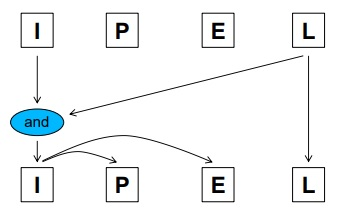
\includegraphics[width=0.4\textwidth]{img/OB-1_0.jpg}
		
		\item systém kontroluje, zda je odpovídající právo obsaženo v množině E
	\end{itemize}
	\item RBAC:
	\begin{itemize}
		\item Role Based Access Control
		\item uživatelé mají přiřazené role
		\item role mají vlastnosti jako uživatelé, ale nelze se přihlásit přímo, pouze přes "su" --- např role root
		\item uživatel se pro použití práv role musí přihlásit (musí tedy mít roli přiřazenou, a zároveň znát její heslo)
		\item role mají přiřazené profily
		\item profily mají přiřazené množiny příkazů, spustitelné pod určitými identitami a se specifickými právy
	\end{itemize}
	\item PAM
	\begin{itemize}
		\item Pluggable Authentication Modules
		\item moduly pro autentizaci, které se dají připojit ke každému programu zvlášť
		\item možnost vytvářet programy nezávisle na konkrétních autentizačních postupech
		\item konfigurace pro konkrétní program: typ modulu --- typ použití --- modul
		
		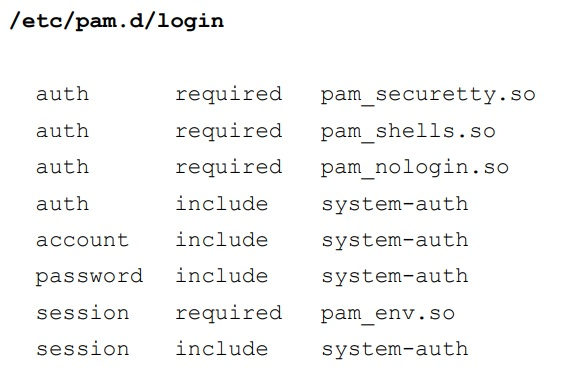
\includegraphics[width=0.6\textwidth]{img/OB-1_1.jpg}
	\end{itemize}
\end{itemize}